\documentclass[a4paper, 14pt]{article}
\usepackage[utf8]{inputenc}
\usepackage[russian]{babel}
\usepackage{graphicx}
\usepackage{listings}
\usepackage{color}
\usepackage{amsmath}
\usepackage{pgfplots}
\usepackage{url}

\usepackage{titlesec}
\titleformat*{\section}{\LARGE\bfseries}
\titleformat*{\subsection}{\Large\bfseries}
\titleformat*{\subsubsection}{\large\bfseries}
\titleformat*{\paragraph}{\large\bfseries}
\titleformat*{\subparagraph}{\large\bfseries}

\usepackage[
backend=biber,
style=alphabetic,
sorting=ynt
]{biblatex}
\addbibresource{lab01.bib}
\bibliography{lab01}

\begin{document}
	\begin{titlepage}
		\begin{center}
			\begin{LARGE}
				Отчет по лабораторной работе №1\\
				по курсу "Анализ алгоритмов"\\
				по теме "Расстояние Левенштейна"
			\end{LARGE}
			
			\begin{Large}
				\vspace{10cm}
				Студент: Барсуков Н.М. ИУ7-56\\
				Преподаватель: Волкова Л.Л.,
				Строганов Ю.В.
			\end{Large}
		\end{center}
	\end{titlepage}

	\tableofcontents
	
	\newpage	
	\section{Аналитическая часть}
	
	\subsection{Постановка задачи}
	
	Изучить, реализовать и сравнить три версии алгоритма Левенштейна поиска минимального редакционного расстояния
	
	\begin{enumerate}
		\item Рекурсивный алгоритм с тремя операциями (вставки, удаления, замены)
		\item Итеративный алгоритм с тремя операциями
		\item Итеративный алгоритм с четырьмя операциями (обмен двух соседних букв)
	\end{enumerate}

	\subsection{Описание алгоритма}
	
	Расстояние Левенштейна (также редакционное расстояние или дистанция редактирования) между двумя строками в теории информации и компьютерной лингвистике — это минимальное количество операций вставки одного символа, удаления одного символа и замены одного символа на другой, необходимых для превращения одной строки в другую.\\
	
	Каждая операция имеет свою оценку штрафа
	
	\begin{enumerate}
		\item Вставка в S1 (I) - 1
		\item Удаление из S1 (D) - 1
		\item Замена символа в S1 (R) - 1
		\item Совпадение символов в S1 и S2 - 0
	\end{enumerate}
	
	\newpage
	\section{Конструкторский раздел}
		
	\subsection{Алгоритм}

	Допустим,что существует две строки S1 и S2 над некоторым алфавитом. Длина одной из них - M, второй - N. Для нахождения расстояния Левенштейна между ними D(S1, S2) можно применить следующую формулу (D(S1, S2) == D(M, N))\cite{Afanasyev92}:
	
	\[
	D(i,j)=\begin{cases}
	max(i,j)\ if\ min(i,j) == 0\\
	min\begin{cases}
	D(i,j-1) + 1\\
	D(i-1,j) + 1\\
	D(i-1,j-1) + (S1[i] <> S2[j])
	\end{cases}
	\end{cases}
	\]
	
	Для случая с 4 операциями формула принимает следующий вид\cite{Vasylenko92}:
	
	\[
	D(i,j)=\begin{cases}
	max(i,j)\ if\ min(i,j) == 0\\
	min\begin{cases}
	D(i,j-1) + 1\\
	D(i-1,j) + 1\\
	D(i-1,j-1) + (S1[i] <> S2[j])\\
	D(i-2,j-2) + 1
	\end{cases} \ if \ i,j>1\\
	min\begin{cases}
	D(i,j-1) + 1\\
	D(i-1,j) + 1\\
	D(i-1,j-1) + (S1[i] <> S2[j])
	\end{cases}
	\end{cases}
	\]
	
	\subsubsection{Итеративный алгоритм}
	\begin{figure}
		\centering
		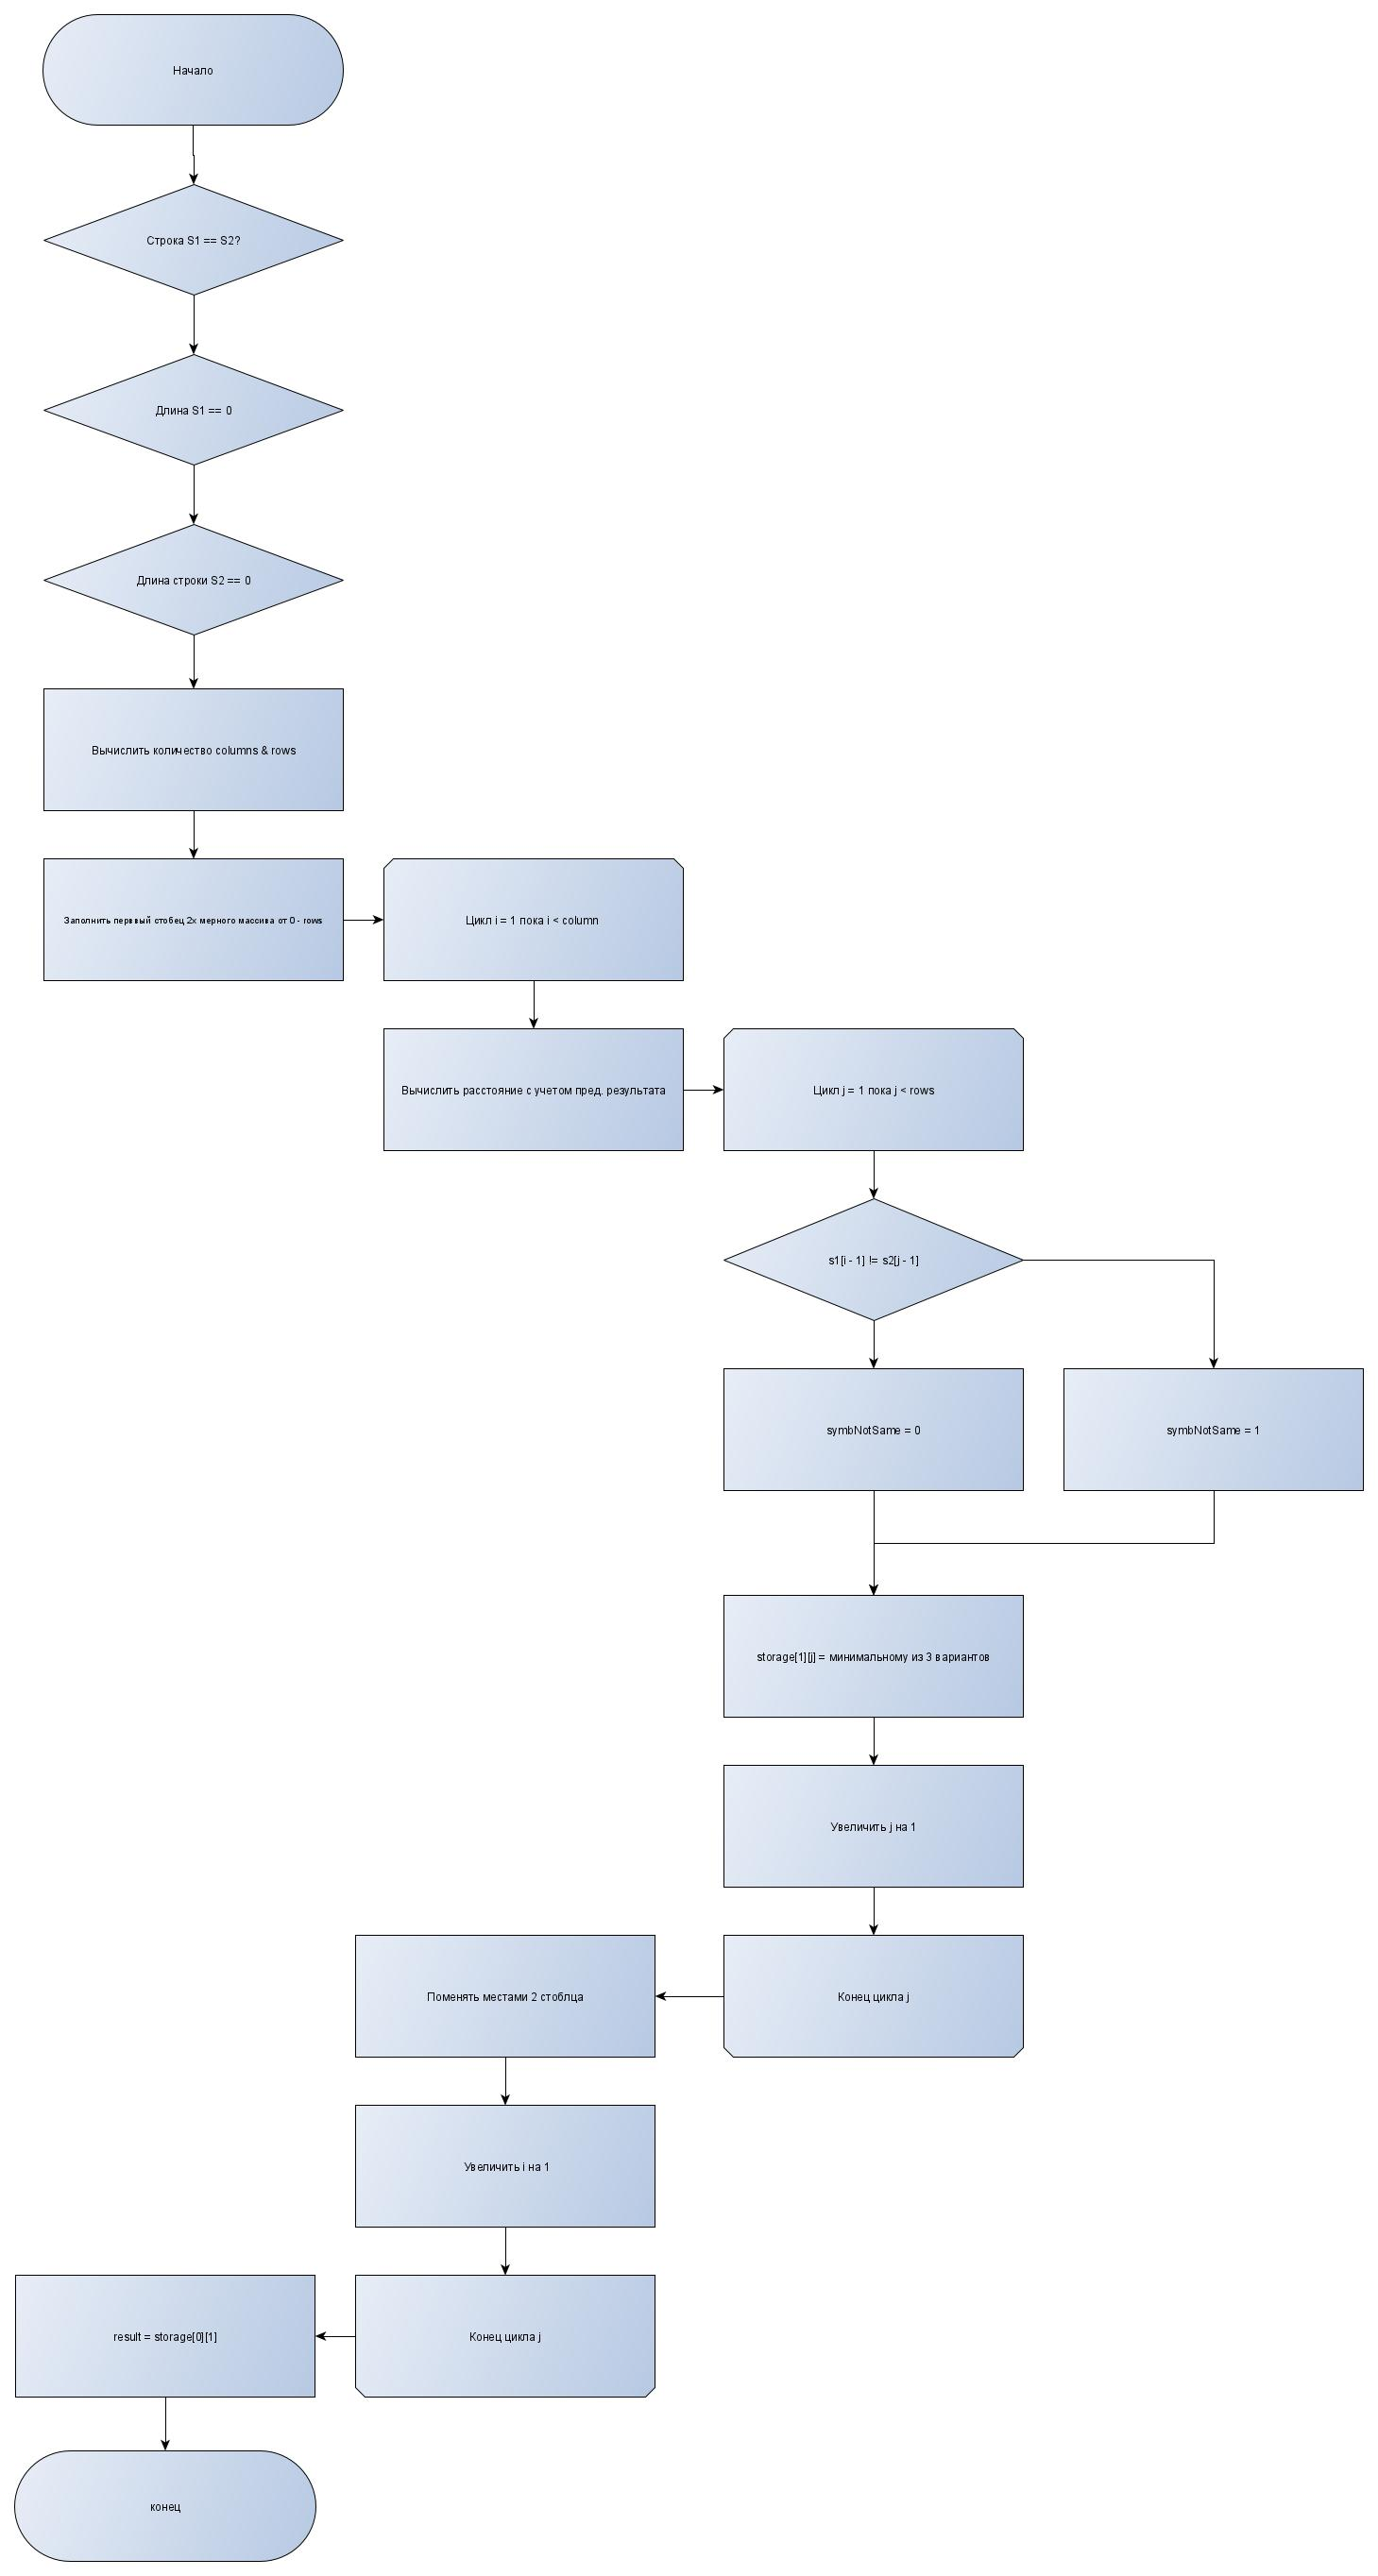
\includegraphics[width=0.7\linewidth]{img/2}
		\caption{Блок схема итеративного алгоритма}
		\label{fig:2}
	\end{figure}
	
	
	\subsubsection{Рекурсивный алгор}
	\begin{figure}[]
		\centering
		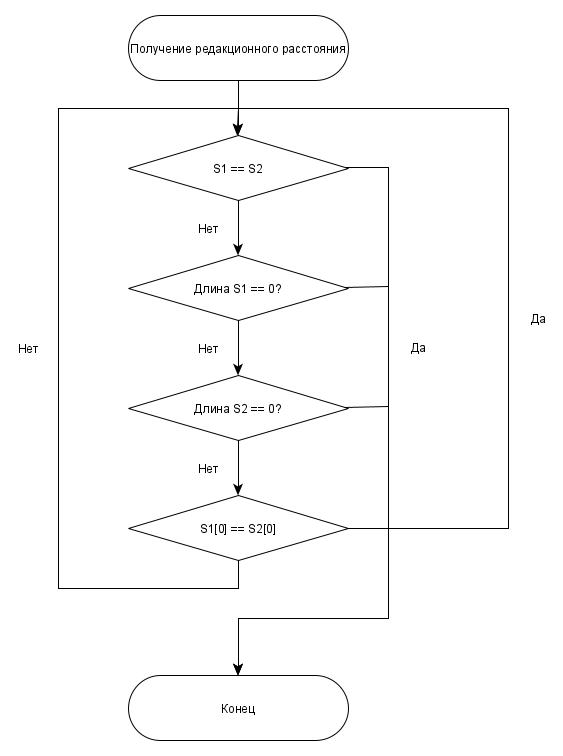
\includegraphics[width=0.7\linewidth]{img/1}
		\caption{Блок схема рекурсивного алгоритма}
		\label{fig:1}
	\end{figure}
	
	
	\subsection{Типы и структуры данных}
	
	\begin{enumerate}
		\item Слова хранятся в виде массивом типа char
		\item Результат хранится в виде целового типа int

	\end{enumerate}

	\subsection{Структура программы}
	
	Пользователя просят выбрать один из двух предоставленных режимов работы
	
	\begin{enumerate}
		\item 1) Поиск редакционного расстояния на 2 строках введенных пользователем
		\item 2) Поиск редакционного расстояния на 2 случайных сгенерированных строках указанной длины
	\end{enumerate}
	
	\newpage
	\section{Технологический раздел}
	
	\subsection{Требования}
	
	Данный программный продукт должен возвращать конечному пользователю редакционное расстояние между 2 строк. Редакционное растояние - это количество операций необходимое для преобразование одной строки в другую.

	
	\subsection{Выбор языка и среды разработки}
	
	Для решения данной поставленной задачи, мной был выбран язык с++ по причине быстродействия, по скольку в нашем случаи пользователю необоходимо как можно быстрее получить результат выполенния нашего алгоритма.
	
	Так же мной используются среда разработки под названием VS Visual Studio по причине удобства и функциональности. И так же желания изучить данную среду по лучше.
	
	\subsection{Интерфейс}
	
	Интерфейс представляет из себя простую консоль в котором пользователь взаимодействует с помощью ввода команд. Такой тип взаимодействия выбран, по причине простоты разработки и удобства тестирования программы
	
	\subsection{Листинг}
	
	\subsubsection{Итеративный Левенштейн}
	
	\begin{lstlisting}
	"int levenstain3(char* str1, char* str2) {
	
	if (strcmp(str1, str2) == 0) {
	return 0;
	}
	
	if (strlen(str1) == 0) {
	return strlen(str2);
	}
	
	if (strlen(str2) == 0) {
	return strlen(str1);
	}
	
	unsigned columns = strlen(str1) + 1;
	unsigned rows = strlen(str2) + 1;
	
	int* storage[2];
	storage[0] = new int[rows];
	storage[1] = new int[rows];
	
	for (unsigned i = 0; i < rows; i++) {
	storage[0][i] = i;
	}
	
	for (unsigned i = 1; i < columns; i++) {
	storage[1][0] = storage[0][0] + 1;
	for (unsigned j = 1; j < rows; j++) {
	bool symbNotSame = false;
	if (str1[i - 1] != str2[j - 1]) {
	symbNotSame = true;
	}
	
	storage[1][j] = min(min(
	storage[0][j] + 1, storage[1][j - 1] + 1), 
	storage[0][j - 1] + symbNotSame);
	}
	swap(storage[0], storage[1]);
	}
	
	int result = storage[0][rows - 1];
	
	delete storage[0];
	delete storage[1];
	
	return result;
	}"
	\end{lstlisting}

	\subsubsection{Левенштейн рекурсивный}
	
	\begin{lstlisting}
	"int levenstainRec3(char* str1, char* str2) {
	
	if (strcmp(str1, str2) == 0) {
	return 0;
	}
	
	if (strlen(str1) == 0) {
	return strlen(str2);
	}
	
	if (strlen(str2) == 0) {
	return strlen(str1);
	}
	
	
	bool symbNotSame = false;
	if (*str1 != *str2) {
	symbNotSame = true;
	}
	
	int result = min(min(levenstainRec3(str1 + 1, str2) + 1, levenstainRec3(str1, str2 + 1) + 1), 
	levenstainRec3(str1 + 1, str2 + 1) + symbNotSame);
	
	return result;
	}"
	\end{lstlisting}

	\subsubsection{Левенштейн модифицированный}
	
	\begin{lstlisting}
	int levenstain4(char* str1, char* str2) {
	
	unsigned lenstr1 = strlen(str1);
	unsigned lenstr2 = strlen(str2);
	
	if (lenstr1 < 2 || lenstr2 < 2)
	return levenstain3(str1, str2);
	
	
	unsigned rows = lenstr1 + 1;
	unsigned columns = lenstr2 + 1;
	
	int* storage[3];
	for (int i = 0; i < 3; i++)
	storage[i] = new int[rows];
	
	for (unsigned i = 0; i < rows; i++) {
	storage[0][i] = i;
	}
	
	storage[1][0] = 1;
	for (unsigned i = 1; i < rows; i++) {
	bool sumbNotSame = false;
	if (str2[i - 1] != str1[0]) {
	sumbNotSame = true;
	}
	storage[1][i] = min(min(storage[1][i - 1] + 1, storage[0][i] + 1), storage[0][i - 1] + sumbNotSame);
	}
	
	for (unsigned i = 2; i < columns; i++) {
	storage[2][0] = storage[1][0] + 1;
	bool symbNotSame = false;
	
	if (str2[0] != str1[i - 1]) {
	symbNotSame = true;
	}
	
	storage[2][1] = min(min(storage[2][0] + 1, storage[1][1] + 1), storage[1][0] + symbNotSame);
	
	for (unsigned j = 2; j < rows; j++) {
	symbNotSame = false;
	if (str2[i - 1] != str1[j - 1]) {
	symbNotSame = true;
	}
	
	storage[2][j] = min(min(min(
	storage[1][j] + 1, storage[2][j - 1] + 1),
	storage[1][j - 1] + symbNotSame),
	storage[0][j - 2] + 1);
	}
	
	swap(storage[0], storage[1]);
	swap(storage[1], storage[2]);
	}
	
	int result = storage[1][rows - 1];
	
	delete storage[0];
	delete storage[1];
	delete storage[2];
	
	return result;
	}
	\end{lstlisting}
	
	
	
	\newpage
	\section{Исследовательский раздел}
	
	\subsection{Сравнение}
	
	\subsubsection{Общие результаты замеров}
	
	Данная таблица содержит в себе общие результаты замеров времени, необходимого для вычисления
	редакционного расстояния между 2 строками равной длины. \\
	Считается что слова полностью различны. \\
	Время измеряется в секундах \\
	На каждый метод берется 100 итераций вычисления \\
	
	\begin{tabular}{|c | c | c | c | c |}
		\hline 
		LEN	& Рекурсивный & Итеративаный & Модифицированный \\
		2 & 0.000105387 & 0.000169814 & 0.000147626 \\
		4 & 0.00224298 & 0.000243199 & 0.0003136 \\
		6 & 0.0621811 & 0.000329813 & 0.000431786 \\
		8 & 1.87619 & 0.000616959 & 0.000716373 \\
		10 & 56.2996 & 0.000702292 & 0.00151893 \\
		\hline
	\end{tabular}
	
	Исходя из полученных данных, сравнение Рекурсивного метода на строках длинее 8 не имеет смысла, по скольку время выполнения растет экспоненциально. Но как мы можем заметить на строках 2 рекурсивный работает на 0,000064 быстрее итеративного и на 0.00042 быстрее Модифицированного.
	
	\subsubsection{Детальное сравнение}
	
	Сравним детально время работы классического Левенштейна и модифицированого (с операцией перестановки). На каждый метод берется среднее время 1000 прогонов. \\
	
	\begin{tabular}{|c | c | c |}
		L & Итеративаный & Модифицированный \\
		\hline
		10 & 6.322e-06 & 1.112e-05 \\
		100 & 0.000724276 & 0.00859501 \\
		200 & 0.00286479 & 0.00383968 \\
		300 & 0.00517626 & 0.00711481 \\
		400 & 0.0091726 & 0.0121067 \\
		500 & 0.0151016 & 0.0191977 \\
		1000 & 0.0540165 & 0.0753726 \\
		2000 & 0.248242 & 0.319514 \\
		3000 & 0.480696 & 0.696582 \\
		\hline
	\end{tabular}
	
	
	\newpage
	\section{Вывод}
	Рекурсивный алгоритм при более простой реализации работает чрезвычайно долго, что делает его использование нецелесообразным. Итеративный алгоритм значительно превосходит его по эффективности.
	Алгоритм с добавленной операцией работает дольше, т.к. имеет более сложную логику, но все равно значительно превосходит по скорости рекурсивный алгоритм.
	
	При этом различие между реализациями тем меньше, чем большая разница длины строк.
	
	\newpage
	\section{Заключение}
	
	В ходе работы было проведено сравнение алгоритмов поиска расстояния Левенштейна (рекурсивной и итеративной реализации) и Дамерау-Левеншнейна (итеративной реализации). Были исследованы зависимости времени выполнения программ, реализующих данные алгоритмы, от искомого расстояния и от размеров строк для случаев с одинаковой длиной исходных строк и случая, когда одна из строк значительно меньше другой. В ходе исследования были сделаны следующие выводы:
	1) Рекурсивная реализация алгоритма Левенштейна выполняется за преемлимое время лишь в случаях, когда размер одной из строк крайне мал (до 10-15 символов)
	2) Итеративные реализации алгоритмов поиска расстояний Дамерау-Левенштейна и Левенштейна имеют схожую ассимптитику, но алгоритм поиска расстояния Дамерау-Левенштейна из-за более сложной внутренней логики в среднем работает медленнее.
	
	\newpage
	\section{Список источников}
	
	\addcontentsline{toc}{chapter}{bibname}

	
	
\end{document}